\documentclass{article}
\usepackage{caption}
\usepackage{subcaption}
\usepackage{amsmath}
\usepackage{amssymb}
\usepackage{mathtools}
\usepackage{array}
\usepackage[margin=0.75in]{geometry}
\usepackage{fancyhdr}
\usepackage{xcolor}
\usepackage{tikz}
\usepackage[normalem]{ulem} % for strike through text
\setlength{\headheight}{0in}

\newcommand{\problemsep}{\leavevmode\\[0.05in] \rule[\baselineskip/4]{\textwidth}{1pt} \\[0.005in] \rule[\baselineskip]{\textwidth}{1pt}\vspace{-\baselineskip/2}\leavevmode\\[0.05in]}
\newcommand{\statementsep}{\leavevmode\\[0.005in] \rule[\baselineskip/4]{\textwidth}{0.4pt}\leavevmode\\[0.005in]}
\pagestyle{fancy}
\rhead{\today}
\lhead{Daniel Mortensen}
\chead{Midterm ``Experience''}

\begin{document}
\noindent \maltese \hspace{1ex} {\bf Sub-Experience One: \emph{Pizza Cutting with 
Lasers}}\\
\noindent **No outside resources, please**
    Given the difficulty of organizing and sequentially lining up cuts to get the 
maximum number of pieces, you invent a laser cutting system that allows you to make
all cuts at once.
    You place $n$ of your devices on the crust with spacing that will maximize the 
number of pieces made and, once activated (ideally remotely because they are 
dangerous), \emph{laser sabers}$^{\circledR}$ shoot between every pair of devices 
simultaneously cutting the pizza into $R(n)$ pieces\footnote{``$R$'' for lase\underline{R}.}.
    Below is an illustration representing $5$ of your devices cutting the pizza 
into $16$ pieces.
\begin{center}
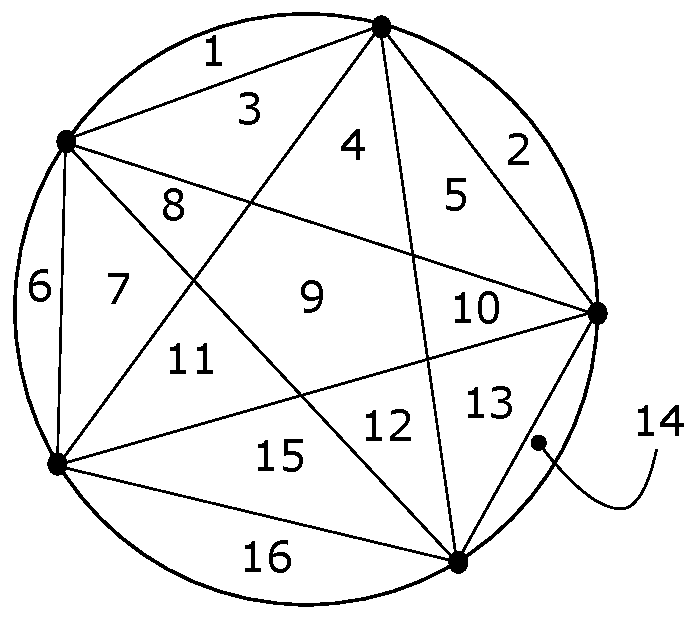
\includegraphics[scale=0.5]{Figures/5pointsOnCircleEx}
\end{center}
\noindent Please determine a formula for $R(n)$.
\statementsep
A new piece is formed when a laser intersects with either another laser, or the edge of the pizza (Fun experiment... try this with Ghostbuster lasers). Each time a `laser' is activated, the number of additional pieces it forms is therefore equal to the number of times it intersects an existing laser plus 1 (as each laser must intersect with the crust at some point) This leads to the expression 
\begin{equation*}
R(n) = \text{nLaser} + \text{nIntersection} + 1
\end{equation*}
where $+ 1$ is necessary because the entire pizza without lines or intersections is considered $1$ piece. A laser can be described as a set of two points, making the the total number of lasers equal to the number of elements in the set of point pairs of which there are $n \choose 2$ elements. Similarly, an intersection can be described as a set of two lasers, or four points, of which there are $n \choose 4$ combinations.  If we substitute these expressions for the number of lasers and the number of intersections into the existing equation, we get
\begin{equation*} \begin{aligned}
R(n) &= {n \choose 2} + {n \choose 4} + 1 \\
	 &= {n \choose 0} + {n \choose 2} + {n \choose 4} \\
     &= \sum_{i=0}^2 {n \choose 2i}
\end{aligned}\end{equation*}
\problemsep
\noindent \maltese \hspace{1ex} {\bf Sub-Experience Two: \emph{Strange Walks}}\\
After the pizza, you decide to take a walk.\\
\noindent {\bf Number of shortest paths using the \emph{city block metric}}.
Starting at Center and Main, you decide to walk to $X$ North and $Y$ East.
The distance is measured in blocks and so the distance from $X_1$ North and $Y_1$ 
East to $X_2$ North and $Y_2$ East is $|X_2 - X_1| + |Y_2 - Y_1|$.
\statementsep
\noindent{\bf SE 2.1.} For yuks, determine $\pi$ in the Logan metric.
Remember that $\pi$ is defined to be the ratio of the circumference to the diameter
of a circle.
And that a circle is the set of points equidistant from a given point (that 
distance is typically called the \emph{radius} of the circle and the point is 
called its \emph{center}.
\statementsep
In this proof, we define circumference as the number of steps it takes to travel to each point that is equidistant fromt the origin. Consider the case where the diameter is 2. The set of all points that are ``on the circle'' is: $\{(1,0), (0,1), (-1, 0), (0, -1) \}$. If we were to walk from one point to the next, beginning at $(1,0)$, then we would walk $8$ blocks, indicating that the circumference is $8$. Because $pi$ is defined as the ratio of circumference to diameter, then 
\begin{equation*}\begin{aligned}
\pi &= \frac{\text{Circumference}}{\text{Diameter}} \\
    &= \frac{8}{2} \\
	&= 4,
\end{aligned}\end{equation*}
indicating that $\pi$ is equal to 4 under the city block metric.
\statementsep
\noindent{\bf SE 2.2.}  Count the number of shortest paths from Center and Main to 
$X$ North and $Y$ East.  A more erudite way to pose this problem is as follows: 
count paths from $(0,0)$ to $(X,Y)$ using steps of the form $R: (x,y) \mapsto 
(x+1,y)$ or $U:(x,y) \mapsto (x,y+1)$.  So paths trace rectilinear ``curves'' in 
the first quadrant of the Cartesian coordinate system that visit only integer-
valued coordinates.
\statementsep
Let $m$ be the number of block to walk in the $y$ direction and $n$ be the number of blocks to walk in the $x$ direction so that $m = \lvert Y \rvert$ and $n = \lvert X \rvert $. A path can be thought of as a linear board with $m + n$ tiles, where each tile is represented by either an $x$ or $y$ square. Note that each path is uniquely defined by only the locations of $x$ or $y$ tiles on the board because any non-x tile must be occupied by a $y$ tile and vice versa. Therefore, the number of board combinations, and by extension the number of possible paths, is described as the number of ways the $x$ tiles can be assigned to $m + n$ locations. Since there are $n$ x tiles, the number of configurations is ${m + n} \choose n$.
\statementsep
\noindent{\bf SE 2.3.}  Walk in strange way.  Start at Center and Main, thinking of
it as the origin $(0,0)$ and take $n$ steps, each of type $R$, $L$, or $U$, with 
$R$ never followed by $L$ and vice-versa. The steps are defined via $R:(x,y) \mapsto (x+1,y)$, $L:(x,y) \mapsto (x-1,y)$, and $U:(x, y+1)$.
Determine the number of different paths with $n$ steps.
\statementsep
We will first show that there is a recurrance relation between $s(n)$ and $s(n - 1)$, and then use that relation to derive a closed form solution. There are two key insights that make up the recurrance. For each step, if the previous step was $R$, then your options are $R$ again or $U$.  If the previous step was $L$, the your options are $L$ or $U$.  If the previous step was $U$, then you may take $R$, $L$, or $U$ steps. The first observation is that if we know $s(n)$, then $s(n+1$ will have two paths for each path in $s(n)$, plus one for each path that ended in $U$ so that
\begin{equation*}
	s(n) = 2s(n - 1) + \text{Number of Up Steps}.
\end{equation*}
The second observation is to show that each parent node must yield one $U$ option, but there is one parent node for each option at $s(n - 2)$, yielding
\begin{equation*}
	s(n) = 2s(n - 1) + s(n - 2).
\end{equation*} \\
The next step is to derive a closed form solution from the recurrance relation. Because the number of decisions for $n$ steps corresponds to the number of leafs a the $n^{\text{th}}$ level of a tree, it is reasonable to assume that the solution is made up of a (collection of) basis function(s) of the form $\gamma^n$, where $\gamma$ represents some constant (similarly to how a tree where each node has two children is described as $2^n$). We the set of possible basis functions as all functions of the form $\gamma^n$ which satisfy the recurrance relation $s(n) = 2s(n - 1) + s(n - 2)$.  We can find the form of gamma by letting $n = 2$, and substituting $\gamma$ in the recurrance relation so that
\begin{equation*}
	\gamma^n = 2\gamma^{n-1} + \gamma^{n - 2}
\end{equation*}
or for $n = 2$, 
\begin{equation*}
	\gamma^2 - 2\gamma - 1 = 0.
\end{equation*}
We can solve for $\gamma$ to get
\begin{equation*}
	\gamma = 1 \pm \sqrt{2}.
\end{equation*}
Because we don't know which basis function will be most effective, we define the solution as their linear combination, where
\begin{equation*}
	s(n) = c_1(1 + \sqrt{2}) + c_2(1 - \sqrt{2}).
\end{equation*}
We can use the results for $n = 0$ and $n = 1$ to solve for the coeffients so that
\begin{equation*}\begin{aligned}
	s(0) &= c_1(1 + \sqrt{2}) + c_2(1 - \sqrt{2}) \\
	s(1) &= c_1(1 + \sqrt{2}) + c_2(1 - \sqrt{2}) \\
\end{aligned}\end{equation*}
which implies that
\begin{equation*}\begin{aligned}
	1 &= c_1(1 + \sqrt{2}) + c_2(1 - \sqrt{2}) \\
	3 &= c_1(1 + \sqrt{2}) + c_2(1 - \sqrt{2}) \\
\end{aligned}\end{equation*}
solving the system of equations yields
\begin{equation*}\begin{aligned}
	c_1 &= \frac{1 + \sqrt{2}}{2} \\
	c_2 &= \frac{1 - \sqrt{2}}{2} \\
\end{aligned}\end{equation*}
so that 
\begin{equation*}
	s(n) = \frac{\left (1 + \sqrt{2} \right )^{n + 1}}{2} + \frac{\left (1 - \sqrt{2} \right )^{n + 1}}{2}
\end{equation*}
\problemsep
\noindent \maltese \hspace{1ex}{\bf Sub-Experience Three: The Master Table of Distributions.} \\
\noindent  Recall the table of distribution functions $f:A \to B$, where $A$ is a 
finite set with $n$ elements and $B$ is a finite set with $x$ elements.
\begin{equation*}
\begin{array}{c|c||c|c|c}
\hline A & B & \mbox{unrestricted }& \mbox{injective}& \mbox{onto} \\ \hline \hline
\mbox{distinguishable} & \mbox{distinguishable} & 1. & 2. & 3. \\ \hline
\mbox{indistinguishable}& \mbox{distinguishable}&4.&5.&6. \\ \hline
\mbox{distinguishable} & \mbox{indistinguishable}& 7. & 8. & 9. \\ \hline
\mbox{indistinguishable}&\mbox{indistinguishable}& 10. &11.&12. \\ \hline 
\end{array}\end{equation*}
\noindent Please determine, with an argument for each, a formula for each entry in 
the table.
\statementsep
In this solution, we consider each entry in the table in reference to its number and give an appropriate response for each in the following list.
\begin{enumerate}
\item Consider the mapping from $A$ to $B$ on an element by element basis. The first element in $A$ can map to any element in $B$, but for the mapping to be a function, each element in $A$ can only map to one element in $B$. Therefore, there are $x^n$ possible mappings between $A$ and $B$ for the unrestricted case. 
\item For a function to be injective, $f(a) = f(b) \implies a = b$, which essentially means that each element in $A$ can only map to one element in $B$. If $\lvert A \rvert > \lvert B \rvert$, then the answer is zero because not all elements in the domain can map to a unique element in the codomain. The following proof is presented for the case where $\lvert A \rvert \le \lvert B \rvert$. Consider an analogy where we place balls (representing elements from the domain) into boxes (representing elements in the codomain). Each matching is counted as a function and we therefore desire to find the number of ways in which to pair the balls from the domain with the boxes from the codomain. Consider the first element from the codomain.  The first element can pair with any of the $x$ elements in the codomain. The second element in the domain can pair with any element in the codomain that is not paired with the first, yielding $x(x - 1)$ combinations. Continuing as such until all elements in the domain have been paired with elements in the codomain yields 
\begin{equation*}
	\text{nCombination} = x(x-1)(x-2)...(x-(n-1))
\end{equation*}
which is equivalent to 
\begin{equation*}
\text{nCombination} = \frac{x!}{(x - n)!}
\end{equation*}
\item A function is surjective if each box contains at least one ball, or more precisely $\forall b \in B, \ \exists a \in A \ni f(a) = b$. We therefore desire to know how many ways the balls can be grouped such that there are $x$ distinct groups. First consider the case where the boxes are unlabeled. When boxes are unlabeled, the question becomes how many ways can we partition n balls into x non-empty groups, which is defined as ${n \brace x}$. Next, consider a scenario where the balls have been partitioned, and how we desire to know how many combinations of partitions exist with labeled boxes. If there are $x$ partitions, then box $a$ would pair with one of $x$ partitions. Box $b$ would pair with one of $x - 1$ partitions and so on until all boxes have paired, yielding $x!$ options. Therefore, for each partitioning, there are $x!$ options which implies that there are a total of ${n \brace x}x!$ functions.
\item Because the elements of $A$ are indistinguishable, each function would differ based on how many elements in $A$ map to each element in $B$. For example, if we use the balls and boxes metaphore, then we would ask how many balls are in each box. Consider a scenario where there were two balls in box 1, three balls in box 2, and 1 ball in box 3. We describe this as an element in a multiset such that 
\begin{equation*}
	f_i = \langle b_1^{(2)}, b_2^{(3)}, b_3^{(1)}\rangle.
\end{equation*}
In general, we refer to the set of all possible functions as the multiset of $B$ size $n$, which has  $\left ( {n \choose x} \right )$ elements, where $n$ is the number of elements from $A$, and $x$ is the number of elements in $B$. Therefore, the number of elements in the multiset of $B$ with size $n$ is ${x + n - 1 \choose x}$. 

\item A function is injective if $f(a) = f(b) \implies a = b$, which can be stated as each ball chooses a single box. However, because the balls are indistinguishable, this amounts to how many ways can I select n of the x boxes, or ${x \choose n}$.
\item Adopting again the ball and boxes metaphore, a surjective function is one where each box contains at least one ball. Because the balls are indistinct, we don't care which ball a box contains. Therefore, assume that the first $x$ balls are placed in individual boxes. Then the number of possible functions is the multiset of $B$ size $n - x$ and consequently, the number of functions is 
\begin{equation*}
	{n - 1 \choose x}
\end{equation*} 
\item A function in this context can be described as one way in which balls (distinguishable) are grouped together, as the boxes are indistinguishable. The set of functions is unrestricted, meaning that the number of groups may range from one to $x$.  The definition of $n$ partition $k$ is the number of ways $n$ objects can be partitioned into $k$ groups.  In this instance, $k$ ranges from $1$ to $x$ so that the number of functions is 
	\begin{equation*}
		\sum_{k=1}^x {n \brace k}
	\end{equation*}
\item An injective function can be thought of as a mapping where each `ball' maps to only one `box'.  If the number of elements in the codomain is less than the number of elements in the domain, than there are zero functions that meet this criteria. Otherwise, let each element from the domain map to a distinct, yet indistinguishable element from the codomain. Because each elemen tin the codomain is indistinguishable, it makes no difference to which codomain element a domain element maps, yielding one function. Another way of thinking of how a function is distinguished is by which elements from the codomain are `grouped' together.  Since all groups will only have one element, then all injective functions are equivalent. \textcolor{red}{What about the definition of injective?  Doesn't this violate that definition because f(a) = f(b) for all elements in the codomain, but a is not equal to b from the domain?}
\item Recall that a function is surjective if $\forall b \in B, \ \exists a \in A \ni f(a) = b$. In a `balls' and `boxes' paradigm, surjective is expressed as a mapping which ensures that all boxes maintain at least one element. This is equivalent to saying that all balls must be divided into $x$ non-empty sets, which is equal to 
	\begin{equation*}
		{n \brace x}
	\end{equation*}
\item Because neither the `boxes' or `balls' are distinguishable, a function's only distinguishing factor is how many balls are mapped to a single box. This can be expressed as a partition of $n$, denoted $p_k(n)$, where $k$ is the number of non-zero partitions (or boxes to which at least one element is mapped). Because the function may map to an arbitrary non-zero number of boxes, the total number of functions is described as
	\begin{equation*}
		\sum_{k=1}^x p_k(n).
	\end{equation*}
\item Because every element in $A$ is equivalent and every element in $B$ is equivalent, then $f(a) = f(b) \implies a = b$ is true for every element in $A$ and $B$. Therefore, every function that maps $A$ to $B$ is injective.
\item The definition of surjective implies that each `box' must to be recipient of at least one `ball'. If we define a function by the number of `balls' that are grouped together as in cell 10, then a surjective function is a function that forms $x$ non-empty sets where the cardinality of all $x$ sets is $n$ which can be expressed as $p_x(n)$, or the partition of $n$ elements into $x$ non-empty sets.
\end{enumerate}
\problemsep
\noindent \maltese \hspace{1ex} {\bf Sub-Experience Four: \emph{Game Time!}}\\
\noindent{\bf SE 4.1: Modified Towers of Hanoi.}  The \emph{Towers of Hanoi} are 
mythical diamond needles, three of them, with $64$ gold discs impaled on one of the
needles.  God told the monks of Brahma to transfer all the discs to another needle 
with the constraints that no larger disc ever be placed atop a smaller disc, and 
only one disc at a time is to be moved.  Once the monks finish moving the discs the
World will end.  Evidently the monks have not yet finished. \\
\noindent Label the needles of the Towers of Hanoi $L$, $M$,
and $R$, for the left, middle, and right, respectively.
Consider the original Towers of Hanoi game,
but with the additional constraint that a disk can only be moved to an adjacent 
peg; that is, a disk can only be moved to $M$ from $L$ or $R$, and can only be 
moved to $L$ or $R$ from $M$.
Assume all discs are initially on $L$.
\statementsep
\noindent \emph{Determine the minimum number of moves (where a \emph{move} is 
defined to be the transfer of one disc from one needle to another) required to 
transfer $n$ discs from $L$ to $R$.}
\statementsep
Let $F_{n}$ be the number of moves it takes to move a set of $n$ discs to the left, or to the right by one. Suppose also that you know $F_{n-1}$ and desire to compute $F_{n}$.  We will demonstrate this proof for the case where we move the stack of tiles from the middle peg to the right peg, but the same logic can be applied for any movement. \\[0.05in]
Because we desire to move the bottom, or $n^{\text{th}}$ tile to the right first, we move the $n-1$ pieces to the left, move the $n^{\text{th}}$ peice to the right, and then move the $n-1$ pieces to the middle, and then right-most needle.  In this transaction, we moved the $n-1$ stack $3$ times, and the $n^{\text{th}}$ piece once.  Therefore, $F_{n} = 3F_{n-1} + 1$, which can be expressed as a sum where
\begin{equation*}\begin{aligned}
F_n &= \sum_{i=0}^{n - 1}3^i.
\end{aligned}\end{equation*}
We desire to find a closed form expression for $F_n$. From the expression above, we know that
\begin{equation*}\begin{aligned}
3F_n - F_n &= 3\sum_{i=0}^{n - 1}3^i - \sum_{i=0}^{n - 1}3^i \\
           &= \sum_{i=1}^n 3^i - \sum_{i=0}^{n-1}3^i\\
		   &= 3^n + \left ( \sum_{i=1}^{n-1}3^i - \sum_{i=1}^{n-1}3^i \right ) - 1 \\
		   &= 3^n - 1
\end{aligned}\end{equation*} 
which also implies that $ 2F_n = 3^n - 1$.
The expression for $F_n$ gives the number of moves to transfer a stack of $n$ pieces from one needle to an adjacent needle. Moving a stack of $n$ pieces from $L$ to $R$ would require two repetitions and so the number of moves it would take transfer $n$ pieces from the $L$ needle to the $R$ is equal to $3^n - 1$.
\statementsep
\noindent \emph{How Long?} Assume the monks of Brahma were given this game with 
$64$ discs, and can move a disc at a rate of one per second. How long in centuries 
will it take for the monks to complete their task?
\statementsep
The number of total moves to relocate a 64 piece stack is $3^{64} - 1 \approx 3.433683820292512\times 10^{30}$ moves, which if done at a rate of 1 move per second implies that it would take approximately $1.088813996794937 \times 10^{21}$ centries to complete.
\problemsep
\noindent {\bf SE 4.2: A Two-Player Game with no Dire Consequences.} \\
\noindent{\bf The Game}\\
\noindent Two players, $A$ and $B$, alternately select an \emph{edge} (line segment
connecting two dots) on the grid graph shown
below and color it red.
The loser of the game is the player who is forced to select an edge that creates
a red $C_4$ --- a red cycle on $4$ vertices.\\
\begin{center}
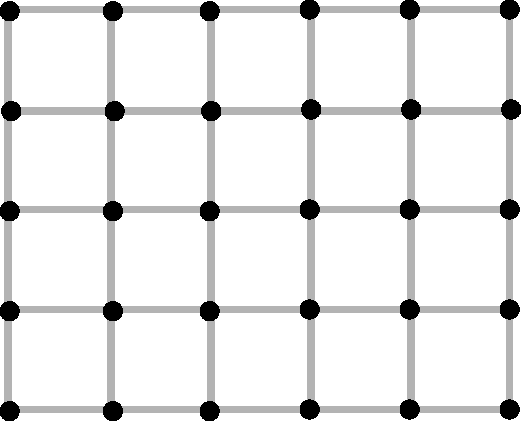
\includegraphics[scale=0.5]{Figures/Saturator_Grid}
\end{center}
\noindent{\bf The Fun}\\
\noindent \emph{Confirm or deny, with proof, whether player $A$ (the first player) 
can always win if she employs a particular strategy for each move.}
\statementsep
This proof shows that the first player can always win if they use the strategy given in this proof. Let each move be denoted $\overline{ab}$, where $a$ and $b$ represent the points to either side of the line. Furthermore, let the grid be numbered starting from (0,0) in the top left corner and incrementing down and to the right where the first element in the pair is the vertical index, and the second is the horizontal. The first move for player 1 must be $\overline{(2,2)(2,3)}$ and then aftward player 1 must mirror player 2's moves about the vertical and horizontal axis. By doing so, player 1 ensures that the board is symmetrical.  If the board is symmetrical, than if player two can find a place to move, then symmetry dictates that player one can as well. By playing the first move directly in the center of the board, player 1 ensures that player two must be the first to select the first element in the symmetric pair. Therefore, the first player to make a choice on a board that has only losing options must be player two, making player one the winner.
\problemsep
\noindent \maltese \hspace{1em} {\bf Sub-Experience Five -- A Matter of Life and 
Death}\\
\noindent **No outside resources**  You are among a group of $n-1$  of your friends
(pretend you have $n-1$ friends even if you don't, where $n$ is possibly very 
large)
and are captured by a horde of theater students who will force you and your $n-1$ 
friends to
enact the play \emph{Cats} with them over and over and over and ... .
Your friends choose death over this fate and decide to
form a circle and have every other person commit suicide (someone has a pistol and 
$n$ bullets,
which is quite reasonable to assume here at USU) until only one person survives, 
who will
supposedly kill themselves.
You want no part of this suicide madness since, you figure, the theater people will
tire eventually and
you can make your escape by taking Jennyanydots hostage with the pistol and 
remaining bullet and escape.\\
\noindent Number you and your friends $1$ to $n$ and assume you all form a vicious 
circle to facilitate the suicide.
\statementsep
\noindent \textsf{Question:} \emph{In which position (call it $S(n)$) must you be 
in order to survive?}\\
\noindent Examples: $S(4) =1$, $S(7) =7$.
\statementsep
We will show that each value for $n$ falls into one of three categories. The first is that $n = 1$, in which case $s(n) = 1$ is trivially satisfied. The second is where $n$ is a power of two. If $n$ is a power of two, then each time the gun traverses the circle, all evenly numbered members will kill themselves and the gun will safely pass by position $1$ like an unholy peace pipe. Hence, if $n$ is a power of $2$, then $s(n) = 1$. The final case is where $n$ is not $1$, and $n$ is also not a power of two ($1$ could be considered a power of two as well, but because $1$ generally causes mayhem in proofs it made more sense to explicitly define the results). Finally, we show that if $n$ is not a power of two, than it's safety position is two higher than that of $n - 1$.
\\ \noindent{\it Claim: } If $n$ is not a powerof two, than the safety position for $n$ members is $2$ more than that of $n - 1$ members.
\\ \noindent{\it Proof: } The movement of the gun is measured by how many positions it traverses. For example, if the gun moves from position 1 to position 3 (skipping the recently deceased person in position 2), than the gun has a movement of two. Define a {\it round} as all gun movement between instances where the gun crosses the $1$ position. Furthermore, define the $n - 1$ scenario as a scenario with $n$ positions where the $n^{\text{th}}$ persion is already dead. For example, consider a comparison between $n = 4$ and $n = 5$. Let the existing positions for the $n = 4$ scenario be given as 
\begin{equation*}
	\langle1, 2, 3, 4, \textcolor{red}{5} \rangle
\end{equation*},
where the fifth position is red to indicate that this person is already dead :) and the existing positions for the $n = 5$ scenario be given as
\begin{equation*}
	\langle 1, 2, 3, 4, 5 \rangle.
\end{equation*}
The sequence the gun travels for the $n - 1$ scenario is given as
\begin{equation*}
\begin{tabular}{c | c | c}
\text{move} & \text{Action} & \text{Number of Steps} \\ \hline
1 $\rightarrow$ 2      & \text{Kill}    & 1 \\
2 $\rightarrow$ 3      & \text{Spare}   & 1 \\
3 $\rightarrow$ 4      & \text{Kill}    & 1 \\
4 $\rightarrow$ 1      & \text{Spare}   & 2 \\
1 $\rightarrow$ 3      & \text{Kill}    & 2 \\
\end{tabular}
\end{equation*}
The gun sequence for the $5$ persion scenario is given as
\begin{equation*}
\begin{tabular}{c | c | c}
\text{move} & \text{Action} & \text{Number of Steps} \\ \hline
1 $\rightarrow$ 2      & \text{Kill}    & 1 \\
2 $\rightarrow$ 3      & \text{Spare}   & 1 \\
3 $\rightarrow$ 4      & \text{Kill}    & 1 \\
4 $\rightarrow$ 5      & \text{Spare}   & 1 \\
5 $\rightarrow$ 1      & \text{Kill}    & 1 \\
1 $\rightarrow$ 3      & \text{Spare}   & 2 \\
3 $\rightarrow$ 5      & \text{Kill}    & 2 \\
\end{tabular}
\end{equation*}
Note how the 5 person scenario contained two more 1-step actions than the 4 person scenario. This will happen generally for all values of $n$ and $n - 1$ because the $n$-person scenario must traverse the extra location, and the $n - 1$ scenario will skip over that location because that person is considered dead, yielding a two step move for the $n - 1$-person scenario. These two additional one-step moves for the $n$-person scenario must include a spare and kill action, which equalizes the number of people between the two scenarios up to that point. Therefore, the number of moves afterward will be equal between the two scenarios and hence, the number of additional steps will also be equal. Therefore, the $n$-person scenario will always have two more steps than the $n - 1$ person scenario, yielding a safety position that is two positions more than the $n - 1$-person scenario.
\\[0.05in] To reiterate, if $n = 1$, than $s(n) = 1$. If $n$ is a power of two, than $s(n) = 1$, otherwise $s(n) = s(n-1) + 2$. To form a final expression for $s(n)$, let $n = 2^k + l$, where $k$ and $l$ are positive integers. The safety position for an $n$-person group is expressed as twice the distance from the nearest power of two, or $2l + 1$. To write the expression explicitely, we have 
\begin{equation*}
s(n) = \left (n - 2^{\lfloor \text{log}_2n \rfloor} \right ) + 1
\end{equation*}

\problemsep
Prove or disprove whether you can order the years 1985,...,1995 so that the resulting number is prime.
\statementsep
Let $N = a_ka_{k=1}...a_1a_0$, where $N$ can also be written in terms of base ten numbers such that
\begin{equation*}
	N = \sum_{i=0}^ka_i10^i.
\end{equation*}
Consider a circle with $11$ steps. If I were to walk $n$ steps around the circle, then I would only pass the $0$ position for every multiple of $11$ (after taking a number of steps that is divisible by $11$). If I take $10$ steps forward along this circle, that is equivalent to taking one step backward (or $-1$ steps). Taking two sets of 10 steps forward is equivalent to $-2$, and so on, where $10$ is equivalent to $-1$ as far as multiplication and addition are concerned. Let us return to the previous expression and substitute each value of $10$ for $-1$, yielding
\begin{equation*}
	N = \sum_{i=0}^ka_i(-1)^i.
\end{equation*}
Note that for each power of 10, the sign alternates from positive 1 to negative 1, resulting in an alternating sum.  If this alternating sum is equal to 0 (think zero-step location), then $N$ is divisible by 11. Select some arbitrary ordering of values 1985 to 1995. Note that each year begins with 19, the next value will either be 8 or 9, and final value ranges from 5 to 5 using single step increments. We can apply the alternating sum as follows: (5 + 6 + 7 + 8 + 9 + 0 + 1 + 2 + 3 + 4 + 5)*(1) + (8 + 8 + 8 + 8 + 8 + 9 + 9 + 9 + 9 + 9 + 9)*(-1) + (9*11)*(1) + (1*11)*(-1). Immediately we can discount the final two sums as they are multiples of 11.  Then observe how (5 + 6 + 7 + 8 + 9 + 0 + 1 + 2 + 3 + 4 + 5) - (8 + 8 + 8 + 8 + 8 + 9 + 9 + 9 + 9 + 9 + 9) = 50 -94 = -44. What we have shown is that if we take $N$ steps forwards in our circular walk, it is equivalent to taking 44 steps backwards, but taking 44 steps backwards will still land the walker at location 1 (the circle doesn't care which direction you travel... 11 steps forward is equivalent to 11 steps backwards), which implies that taking $N$ steps forward is also equivalent to taking {\emph zero} steps forward in our 11-step circle, implyingn that $N$ is divisible by $11$. Hence, $N$ (or any arbitrary ordering of the numbers 1985 to 1995) cannot ever by prime as it is always divisible by 11.
\end{document}
